\section{Propriétés des ondes : réflexion, réfraction. }

Nous avons observé, grâce à la cuve à ondes, ces phénomènes
ondulatoires.

Analysons-les plus en détail.

\subsection{Réflexion des ondes} % (p 62 à 65 du livre)}}

\begin{figure}
\centering
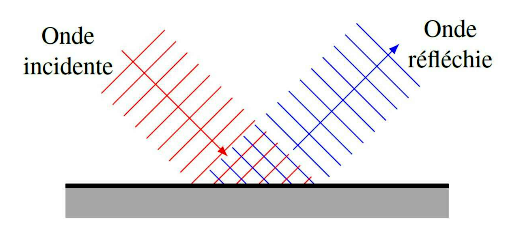
\includegraphics[width=6.957cm,height=3.156cm]{Pictures/100000010000020F000000EF2B8E3664FF7463BF.png}
\caption{}
\end{figure}

Nous l'avons observée à l'aide de la cuve à onde et voyez sur la figure
ci-contre que \textbf{la longueur d'onde est inchangée.}

Sous quel angle est renvoyée l'onde~?

\begin{figure}
\centering
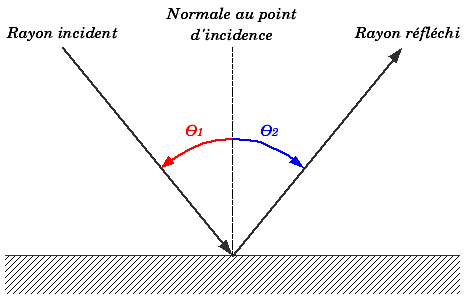
\includegraphics[width=6.548cm,height=4.193cm]{Pictures/10000001000001D10000012A74B1751A93498773.png}
\caption{}
\end{figure}

Définitions~: 
\begin{enumerate}
\item \textbf{L'angle d'incidence ($\theta_i$)} est l'angle formé par la direction
de propagation de l'onde incidente et la normale (la perpendiculaire) à
l'obstacle.
\item \textbf{L'angle de réflexion ($\theta_r$)} est l'angle formé par la direction
des ondes réfléchies et la normale.
\end{enumerate}

Lire les pages 64-65 du livre VANIN, 3è édition de Y. Verbist
\begin{enumerate}
 \item Réflexion d'ondes sonores.
 \item Réflexion sonores dans une salle.
 \item Le sonar
 \item L'échographie
 \item
\begin{figure}
\centering
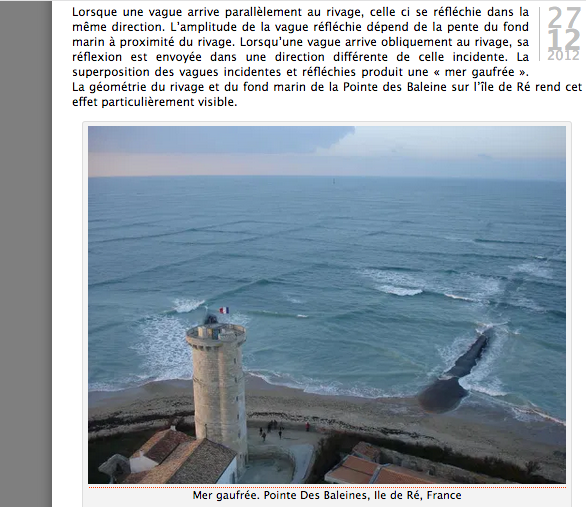
\includegraphics[width=7.13cm,height=5.433cm]{Pictures/100000010000024A000001FB96EDB4A31FE3EFC8.png}
\caption{La mer gaufrée à la pointe des Baleines à l'Ile de Ré, en France.}
\end{figure}
\end{enumerate}

Une belle visualisation des ondes réfléchies est la mer gaufrée.

Nous voyons la superposition des vagues incidentes et des vagues
réfléchies qui produit ``un quadrillage'', appellé ``mer gaufrée'',
particulièrement visible à l'Ile de Ré.

\subsection{Réfraction des ondes} % ( P 66 à 69 du livre)

La \textbf{réfraction} est un phénomène ondulatoire qui est tel
qu'\textbf{une onde change de direction }lorsqu'elle \textbf{change de
milieu}. Ce changement de direction est dû à un changement de vitesse de
l'onde qui traverse deux milieux différents.

\subsection{Analyse expérimentale. }

Pour analyser ce phénomène, prenons une cuve à onde et simulons le
changement de milieu à l'aide d'une modification de la profondeur de
l'eau.

En effet, la vitesse des vagues diminue lorsque la profondeur de l'eau
diminue.

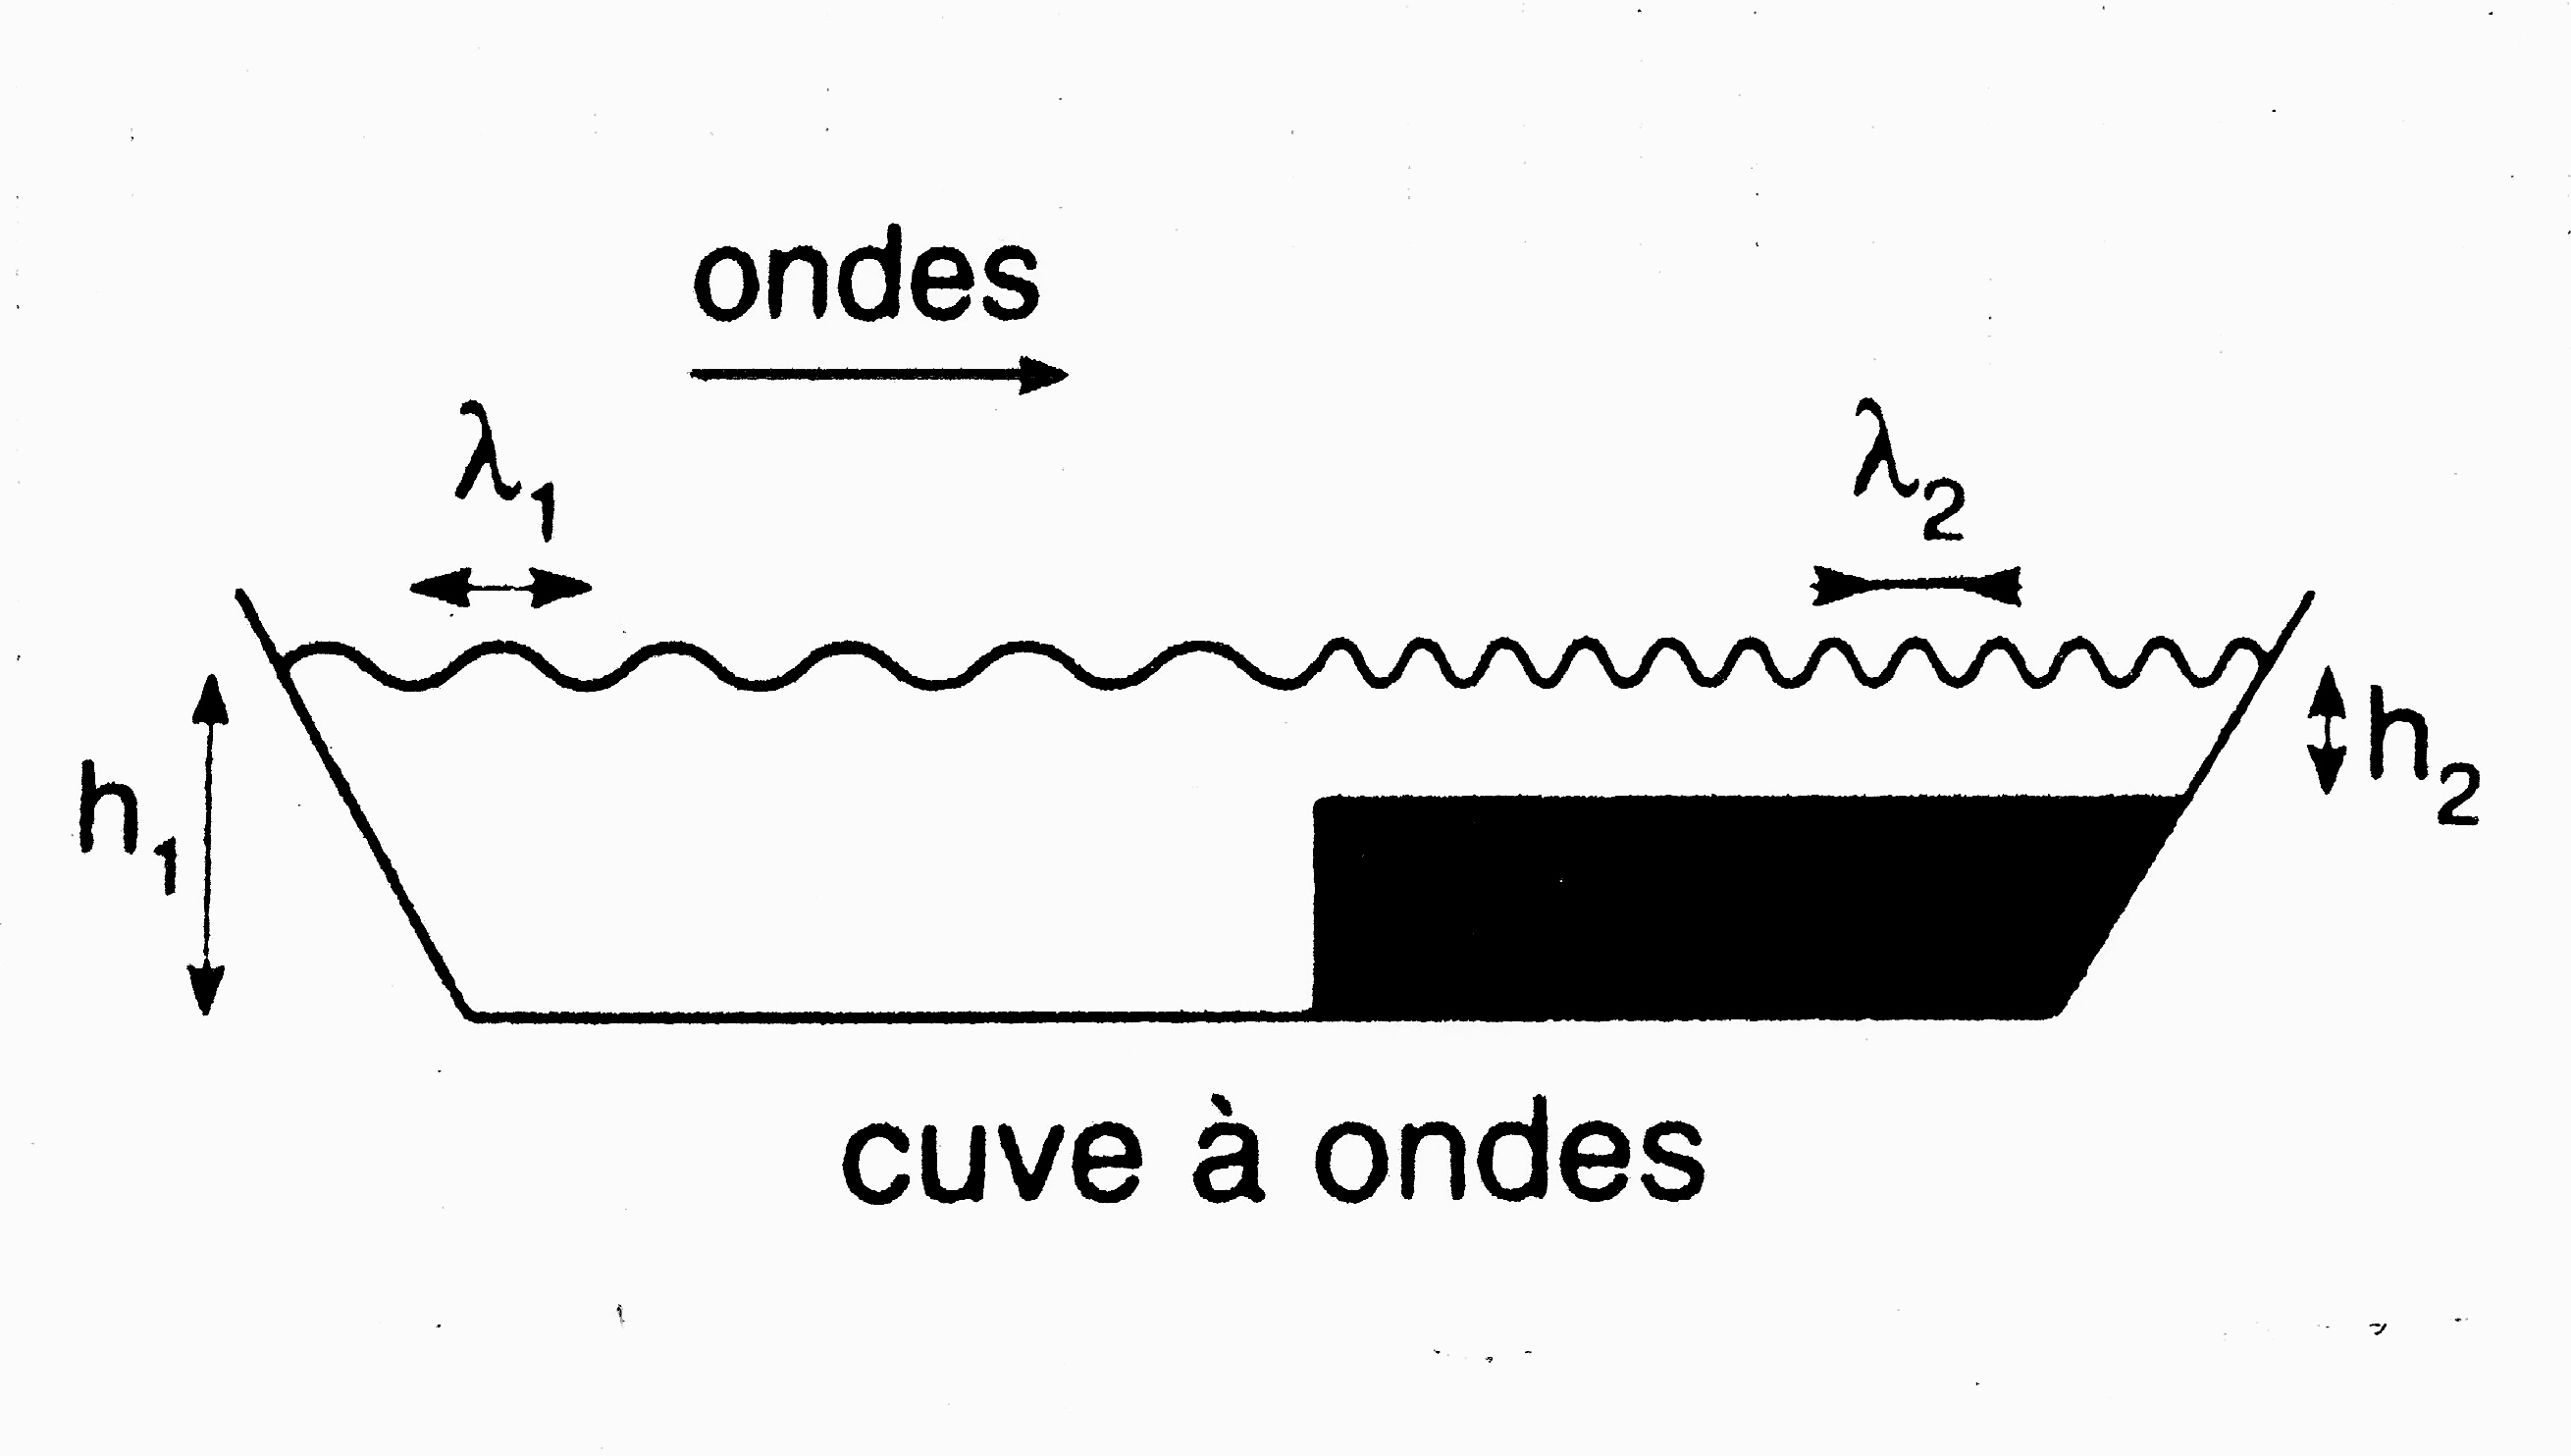
\includegraphics[width=6.017cm,height=3.408cm]{Pictures/1000000100000A3C000005CCA7E68DBE45CF2A53.png}

Nous pouvons observer~:

$h_1 > h_2$ donc $v_1 > v_2$
où $v_1$ est la vitesse de l'onde dans le milieu le plus profond et $v_2$ la
vitesse de l'onde dans le milieu le moins profond.

Et comme $f_1 = f_2$ (la fréquence n'est pas modifiée, c'est la fréquence de
l'OH)~:

FIXME 

La réfraction modifie la vitesse de l'onde en changeant de milieu et
donc modifie dans le même sens la longueur d'onde.

Observons la cuve à onde sous un autre angle, vue de haut (toujours dans
la même situation~: $v_1>  v_2$).

\begin{figure}
\centering
\includegraphics[width=5.076cm,height=4.512cm]{Pictures/1000000100000D3A00000BC4C32708B895F5FFB5.png}
\caption{}
\end{figure}

Comme l'onde passe d'un milieu profond à un milieu moins profond, elles
ralentissent et changent de direction.

Comment quantifier ce changement de direction~?

\begin{figure}
\centering
\includegraphics[width=6.652cm,height=5.652cm]{Pictures/1000000100000D3A00000B3EA693DF6AC5A29F0B.png}
\caption{}
\end{figure}

Définissons les angles d'incidence et de réfraction~:

a) \textbf{L'angle d'incidence (1)} est l'angle formé par la direction
de propagation de l'onde incidente et la normale (la perpendiculaire) à
l'obstacle.

b\textbf{) L'angle de réflexion (2)} est l'angle formé par la direction
des ondes réfractées et la normale.

Nous voyons ci-contre que~:

si v1  v2 alors 1  2 (l'onde se rapproche de la normale).

Quelle est la relation entre les vitesses et les angles d'incidence et
de réfraction~?

\begin{figure}
\centering
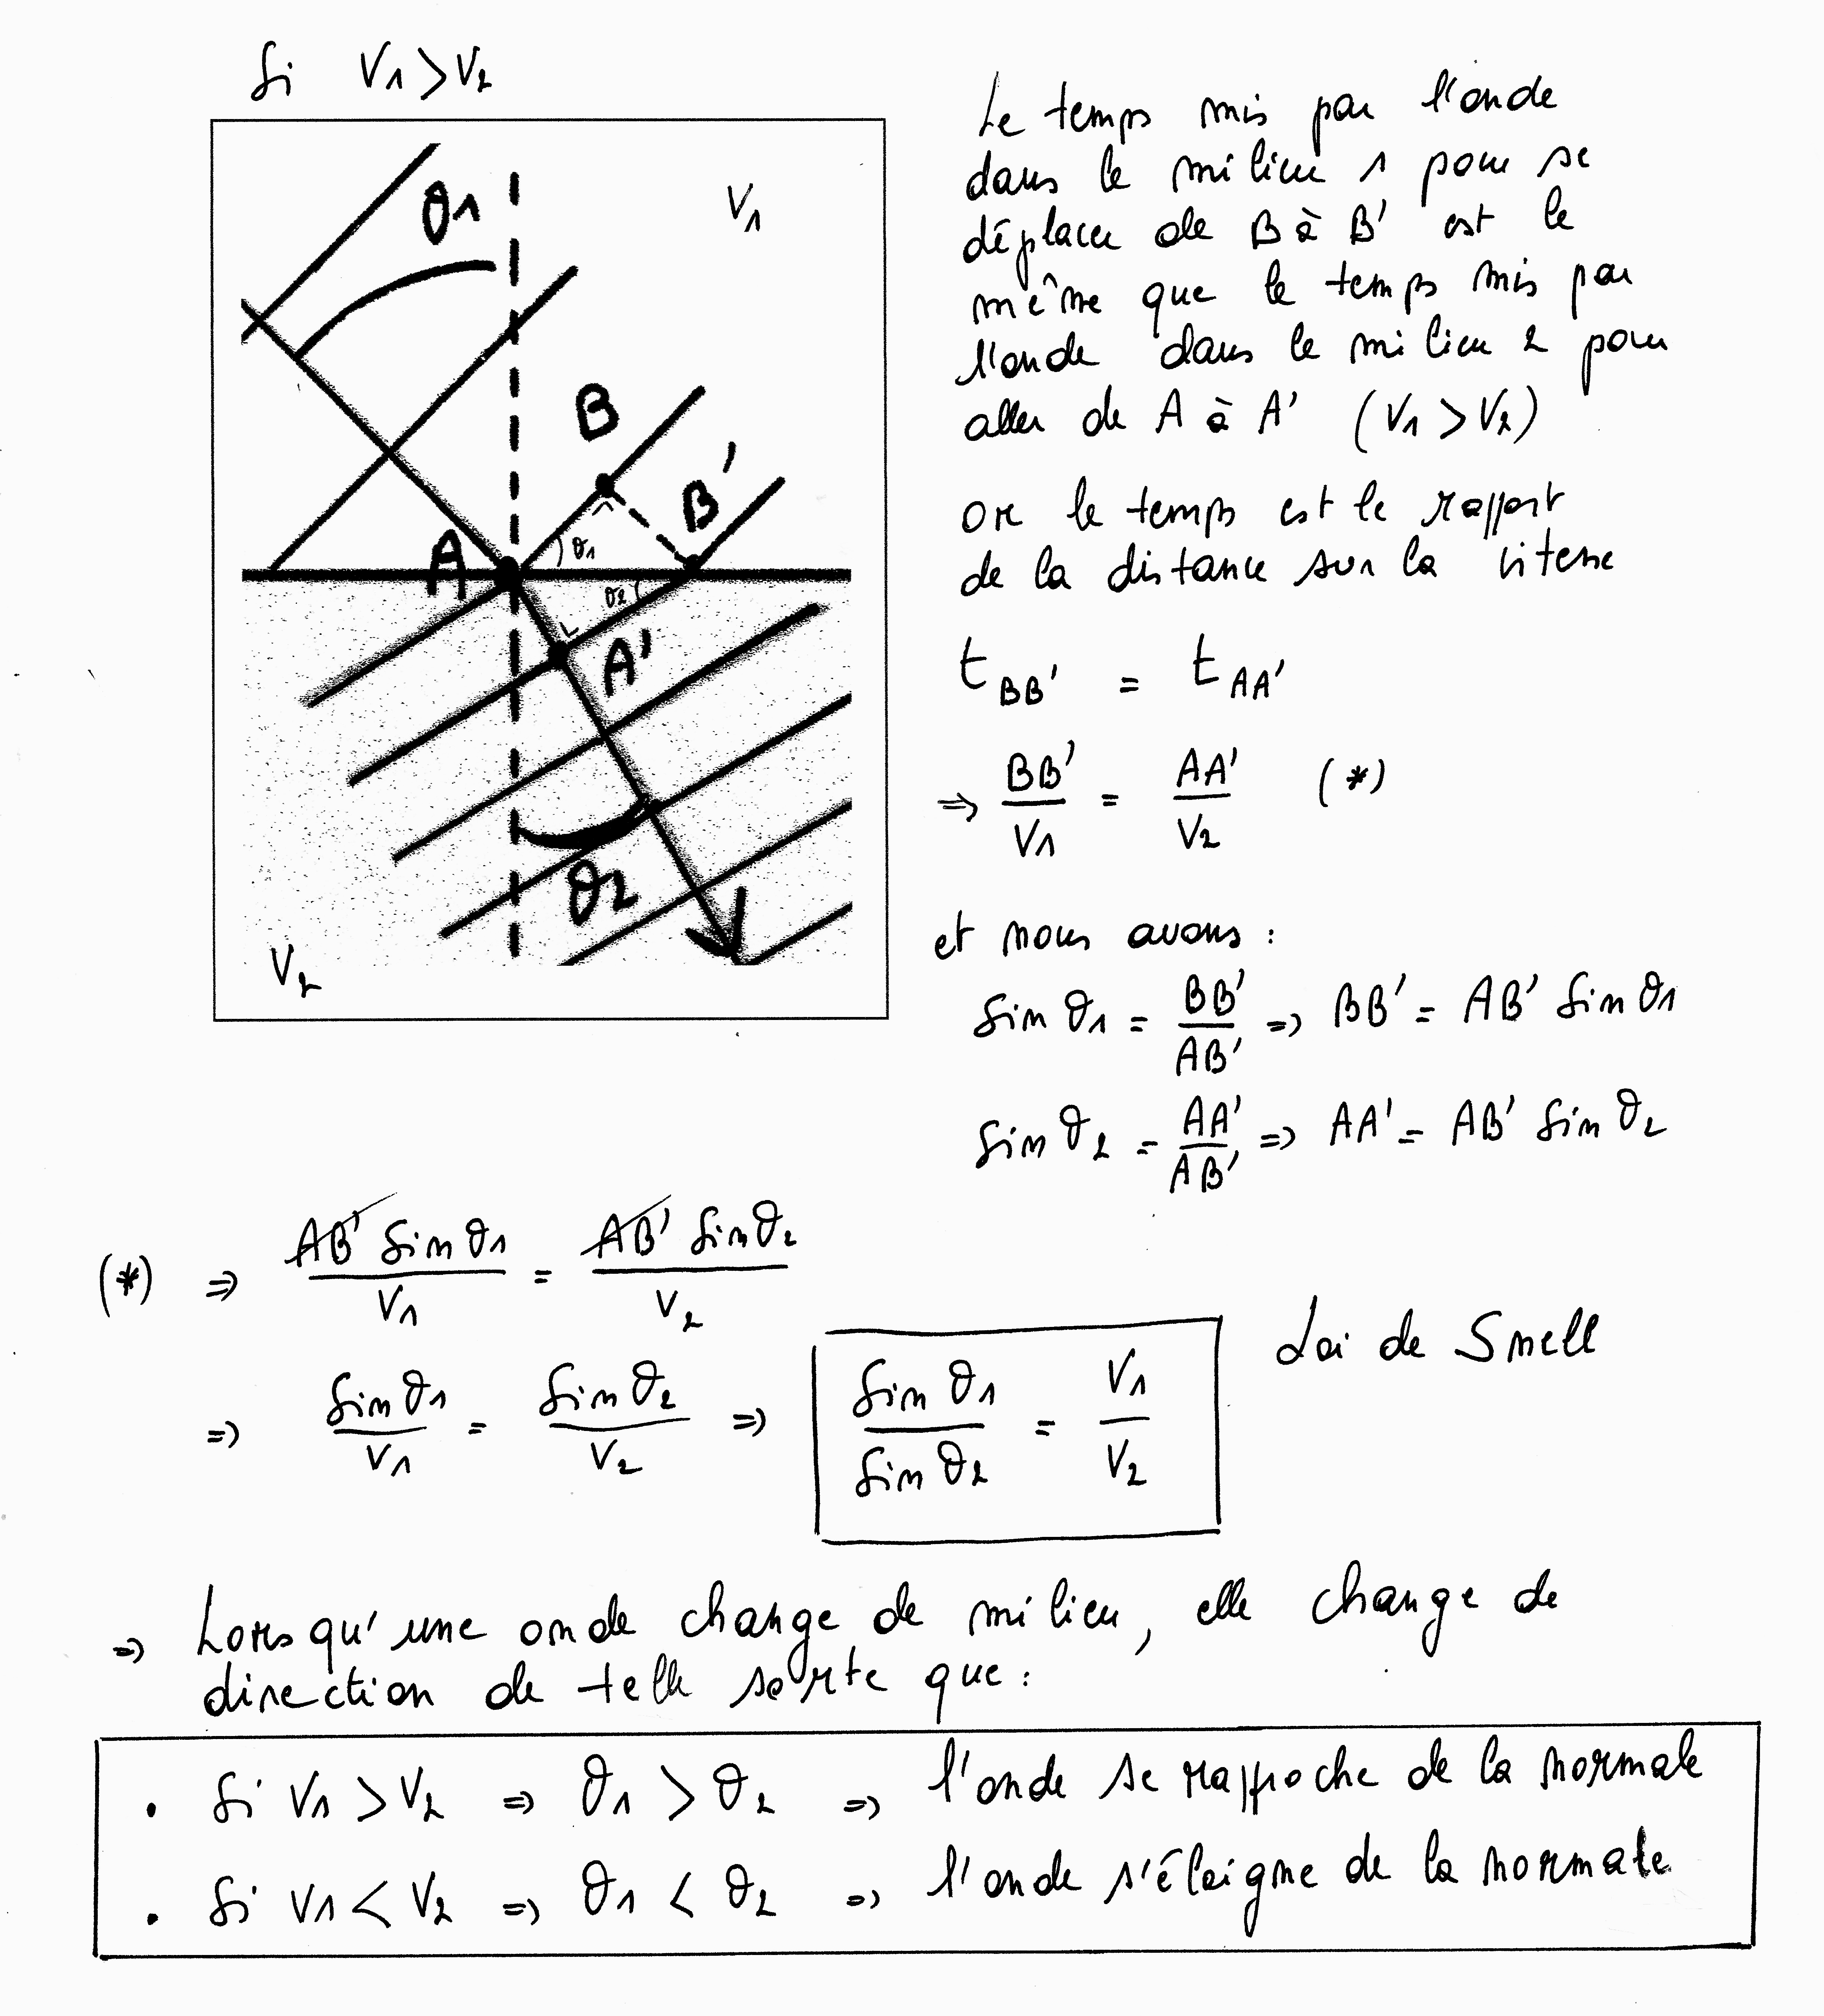
\includegraphics[width=18.516cm,height=20.461cm]{Pictures/10000001000013080000150A74E0EE61F2B1EE2F.png}
\caption{}
\end{figure}

\begin{figure}
\centering
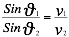
\includegraphics[width=2.634cm,height=1.412cm]{Pictures/1000000100000045000000258E7A9DA5E900B5EA.png}
\caption{}
\end{figure}

\emph{\textbf{Applications de la réfraction}}

\textbf{On sait que le son se propage plus loin la nuit que le jour,
lorsqu'un son est produit au niveau du sol. Pourquoi cette différence~?
}

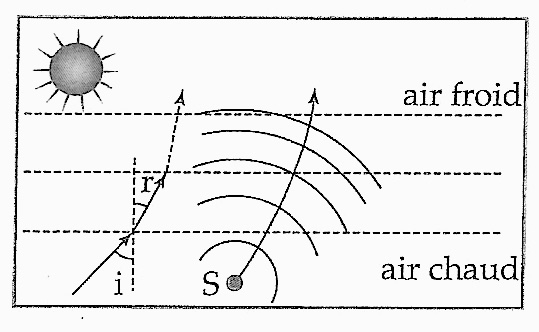
\includegraphics[width=8.356cm,height=5.151cm]{Pictures/100000010000021B0000014C687D75FBC118E240.png}Durant
la journée, la température de l'air diminue quand on s'élève en
altitude. En effet, le sol chauffe plus rapidement que l'atmosphère.

Or, \textbf{la vitesse du son diminue lorsque la température diminue.}

Nous avons vu que lorsque la vitesse d'une onde diminue, l'onde se
réfracte de telle sorte que l'angle de réfraction r soit inférieur à
l'angle d'incidence i.

En traversant différentes couches d'air de plus en plus froides en
s'élevant, le son est dévié vers le haut. Un observateur au sol
n'entendra plus le son.

\begin{figure}
\centering
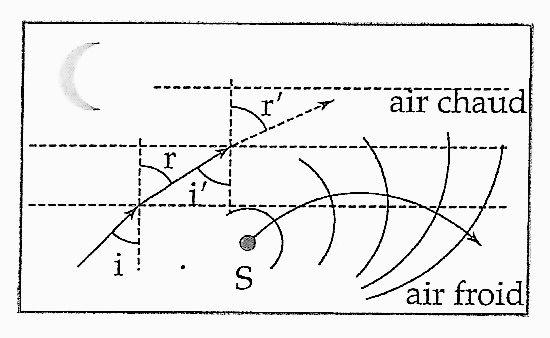
\includegraphics[width=8.414cm,height=5.172cm]{Pictures/1000000100000226000001526F2E95C895BB2EC1.png}
\caption{}
\end{figure}

Durant la nuit, le phénomène inverse se passe. La température de l'air
augmente quand on s'élève. En effet, le sol se refroidit plus vite que
l'atmosphère.

\textbf{La vitesse du son augmente lorsque la température augmente} et
donc la vitesse de l'onde réfractée est plus grande que la vitesse de
l'onde émise. L'angle de réfraction sera plus grand que l'angle
d'incidence et l'onde, étant réfractée vers le sol, se rapproche du sol
et le son porte plus loin.

\emph{\textbf{EXERCICE 1}}

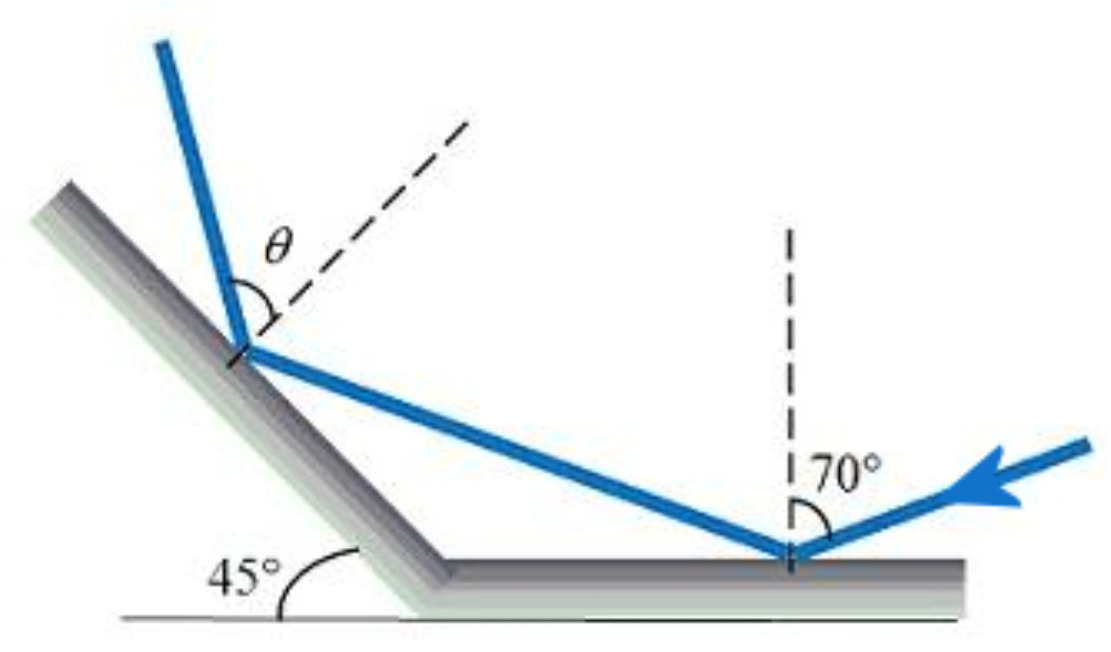
\includegraphics[width=7.807cm,height=4.581cm]{Pictures/10000001000004570000028CCC770E758E0BAEF3.png}Dans
le cadre d'un phénomène de réflexion~: quel est l'angle  sur cette
figure?

(Réponse~: 65°)

\emph{\textbf{EXERCICE 2 ( N° 6 du livre p 78)}}

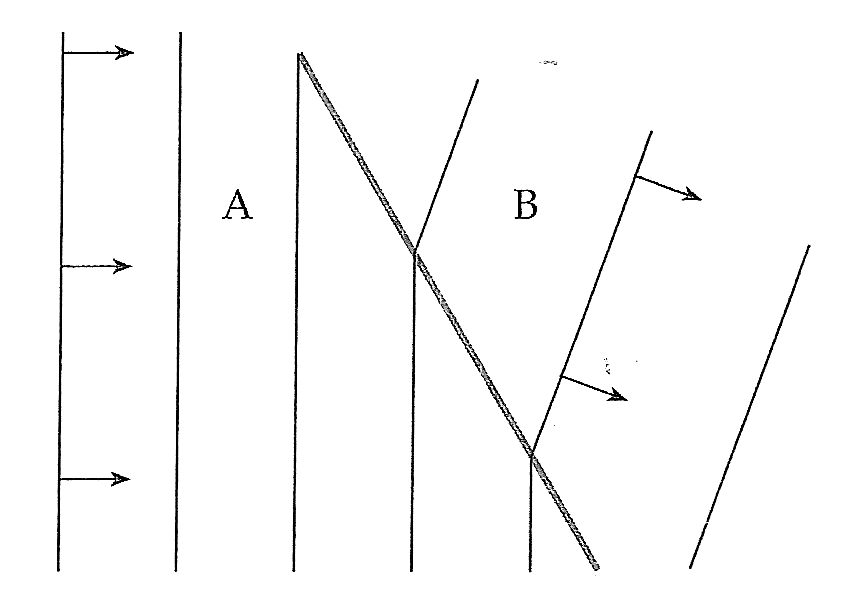
\includegraphics[width=7.086cm,height=4.948cm]{Pictures/10000001000003620000025DC72F2F5C1B5B30DC.png}La
figure ci-contre représente le passage d'une onde d'un milieu A vers un
milieu B.

a) Dans lequel de ces deux milieux la vitesse de propagation est-elle la
plus élevée~?

b) Si la fréquence des ondes est de 50 Hz et que la figure est à
l'échelle 1:1, calculer la vitesse de l'onde dans chaque milieu.

\emph{\textbf{EXERCICE 3}}

Construire le schéma de réfraction d'une onde ayant une vitesse
incidente v1 et une vitesse v2 dans le second milieu, avec \textbf{v1 =
1,5 v2} ; pour les angles d'incidence suivants :

a) i = 10°

b) i = 30 °

c) i = 41,5 °

d) i = 89°

\emph{\textbf{EXERCICE 4}}

Construire le schéma de réfraction d'une onde ayant une vitesse
incidente v1 et une vitesse v2 dans le second milieu, avec \textbf{v2 =
1,5 v1} ; pour les angles d'incidence suivants :

a) i = 10°

b) i = 30 °

c) i = 41,5 °

d) Calculer l'angle limite de réfraction

e) Construire la propagation de l'onde pour un angle d'incidence i = 50
°

\emph{\textbf{EXERCICE 5 (N°8 du livre p 78) }}

Quel est l'angle d'incidence maximal pour qu'une onde sonore émise dans
l'air puisse être réfractée dans l'eau sans subir de réflexion totale à
la surface de l'eau ?

\emph{\textbf{EXERCICE 6 ( N° 7 DU LIVRE P 78)}}

Dans un canal de navigation de 25 mètres de large, une onde; dont la
longueur d'onde est de 1,5 m,; se propage à la vitesse de 2 m/s. Que
devient cette longueur d'onde lorsque l'onde arrive dans une partie
moins profonde du canal où la vitesse de propagation est réduite à 1,6
m/s ?

\emph{\textbf{EXERCICE 7}}

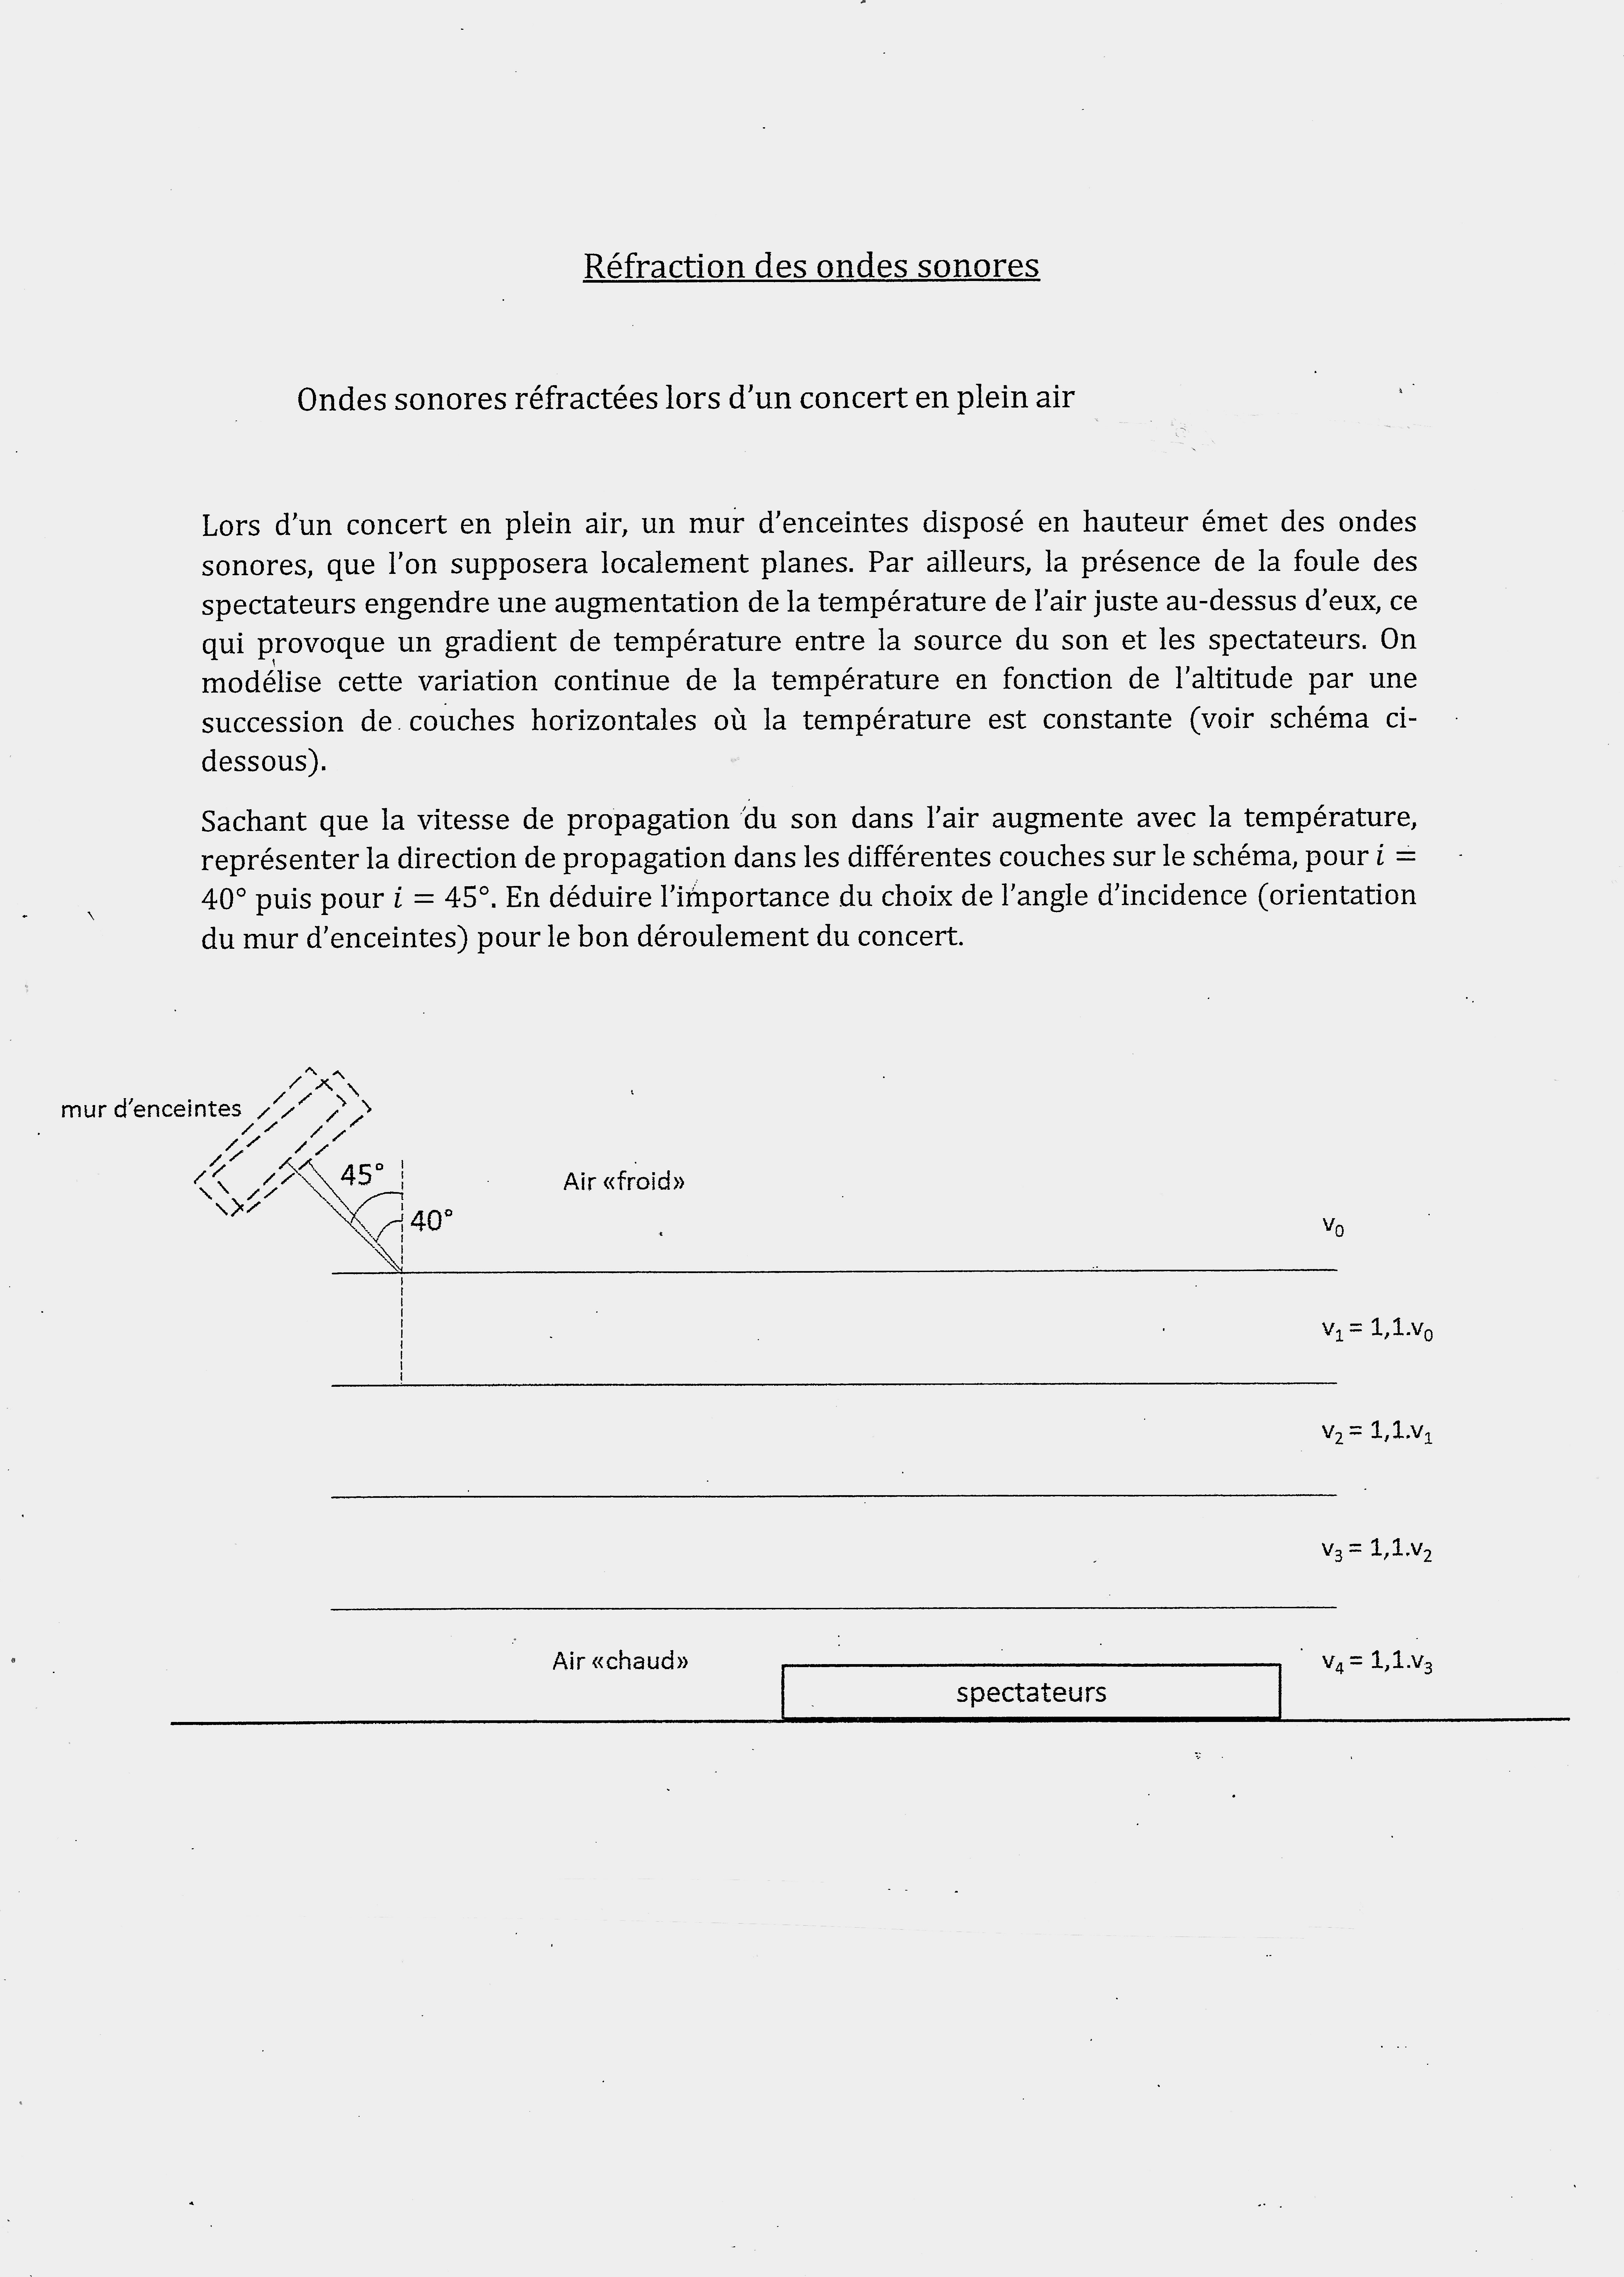
\includegraphics[width=18.501cm,height=21.812cm]{Pictures/100000010000133200001AE8CBE600732ABF4D48.png}

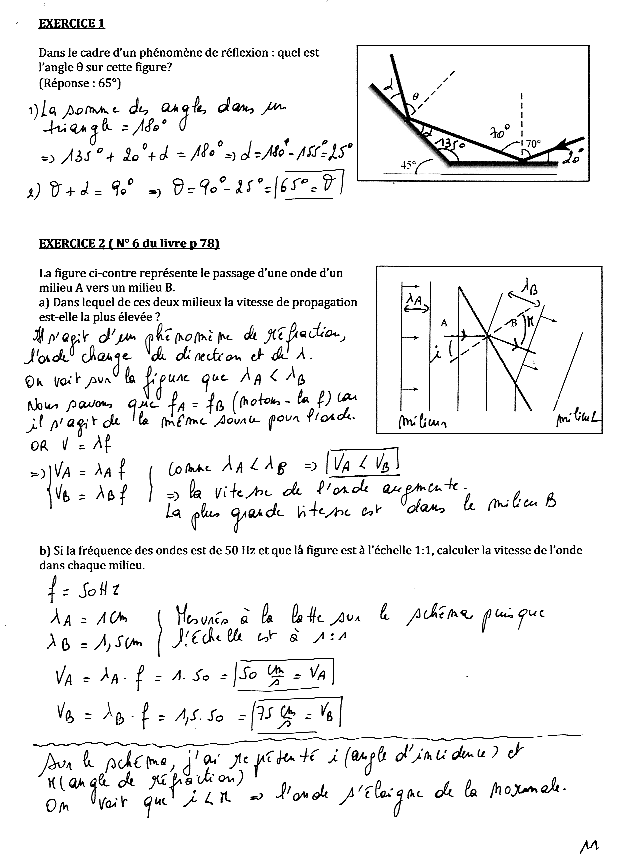
\includegraphics[width=18.501cm,height=25.636cm]{Pictures/100000010000026D0000035C988B6F7E90298C6A.png}

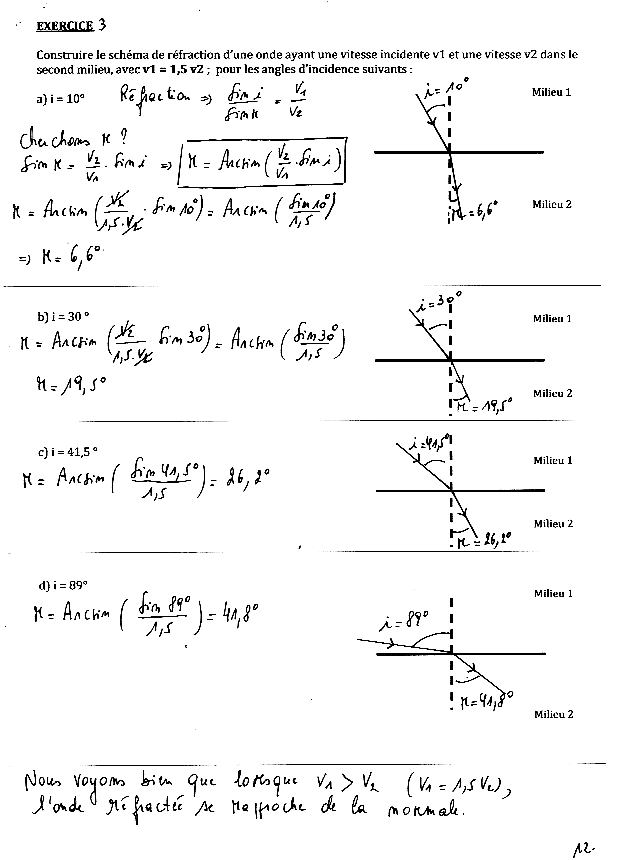
\includegraphics[width=18.501cm,height=25.636cm]{Pictures/100000010000026D0000035C190239246DBF1AB2.png}

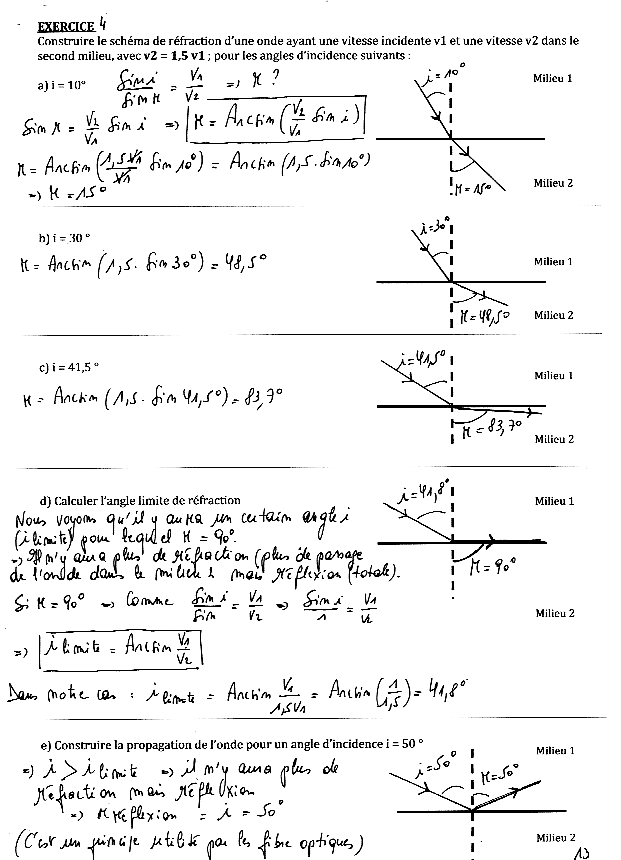
\includegraphics[width=18.501cm,height=25.636cm]{Pictures/100000010000026D0000035CCC97A4EC19D02B04.png}

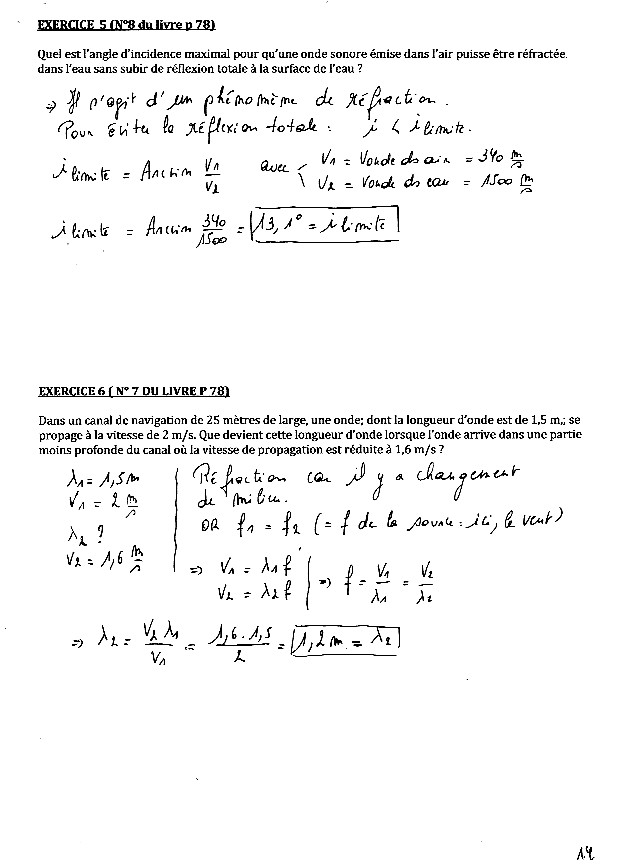
\includegraphics[width=18.501cm,height=25.636cm]{Pictures/100000010000026D0000035CFF0F2F588EBA9209.png}

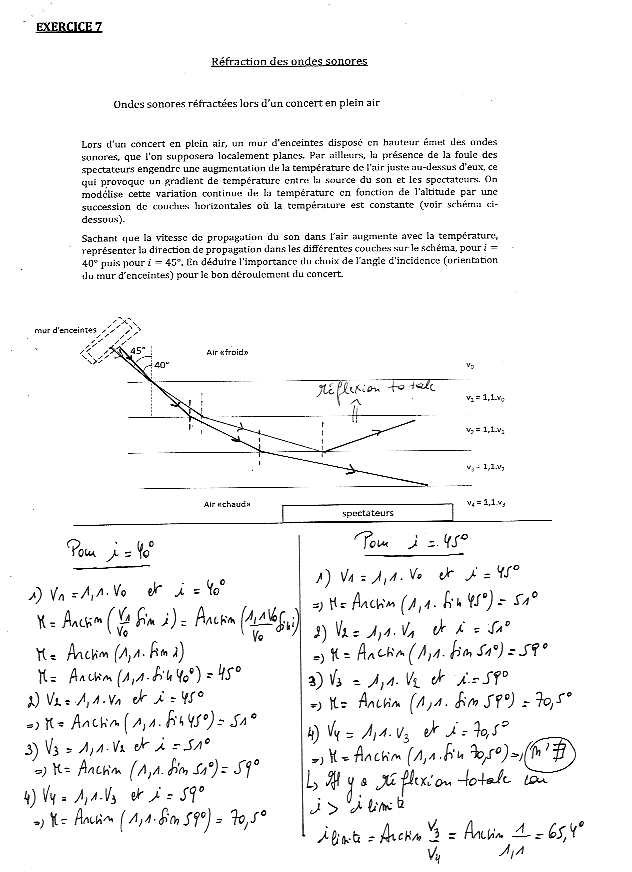
\includegraphics[width=18.501cm,height=25.527cm]{Pictures/1000000100000278000003689DDE3826ADE887B9.png}
